% Options for packages loaded elsewhere
\PassOptionsToPackage{unicode}{hyperref}
\PassOptionsToPackage{hyphens}{url}
\documentclass[
  a4paper, twoside, 10pt, titlepage]{book}
\usepackage{xcolor}
\usepackage[a4paper, left=3.5cm, right=3cm, top=2.5cm,
bottom=3cm]{geometry}
\usepackage{amsmath,amssymb}
\setcounter{secnumdepth}{-\maxdimen} % remove section numbering
\usepackage{iftex}
\ifPDFTeX
  \usepackage[T1]{fontenc}
  \usepackage[utf8]{inputenc}
  \usepackage{textcomp} % provide euro and other symbols
\else % if luatex or xetex
  \usepackage{unicode-math} % this also loads fontspec
  \defaultfontfeatures{Scale=MatchLowercase}
  \defaultfontfeatures[\rmfamily]{Ligatures=TeX,Scale=1}
\fi
\usepackage{lmodern}
\ifPDFTeX\else
  % xetex/luatex font selection
    \setmainfont[]{Palatino}
    \setmonofont[]{Hack Nerd Font Mono Regular}
\fi
% Use upquote if available, for straight quotes in verbatim environments
\IfFileExists{upquote.sty}{\usepackage{upquote}}{}
\IfFileExists{microtype.sty}{% use microtype if available
  \usepackage[]{microtype}
  \UseMicrotypeSet[protrusion]{basicmath} % disable protrusion for tt fonts
}{}
\makeatletter
\@ifundefined{KOMAClassName}{% if non-KOMA class
  \IfFileExists{parskip.sty}{%
    \usepackage{parskip}
  }{% else
    \setlength{\parindent}{0pt}
    \setlength{\parskip}{6pt plus 2pt minus 1pt}}
}{% if KOMA class
  \KOMAoptions{parskip=half}}
\makeatother
\usepackage{color}
\usepackage{fancyvrb}
\newcommand{\VerbBar}{|}
\newcommand{\VERB}{\Verb[commandchars=\\\{\}]}
\DefineVerbatimEnvironment{Highlighting}{Verbatim}{commandchars=\\\{\}}
% Add ',fontsize=\small' for more characters per line
\newenvironment{Shaded}{}{}
\newcommand{\AlertTok}[1]{\textcolor[rgb]{1.00,0.00,0.00}{\textbf{#1}}}
\newcommand{\AnnotationTok}[1]{\textcolor[rgb]{0.38,0.63,0.69}{\textbf{\textit{#1}}}}
\newcommand{\AttributeTok}[1]{\textcolor[rgb]{0.49,0.56,0.16}{#1}}
\newcommand{\BaseNTok}[1]{\textcolor[rgb]{0.25,0.63,0.44}{#1}}
\newcommand{\BuiltInTok}[1]{\textcolor[rgb]{0.00,0.50,0.00}{#1}}
\newcommand{\CharTok}[1]{\textcolor[rgb]{0.25,0.44,0.63}{#1}}
\newcommand{\CommentTok}[1]{\textcolor[rgb]{0.38,0.63,0.69}{\textit{#1}}}
\newcommand{\CommentVarTok}[1]{\textcolor[rgb]{0.38,0.63,0.69}{\textbf{\textit{#1}}}}
\newcommand{\ConstantTok}[1]{\textcolor[rgb]{0.53,0.00,0.00}{#1}}
\newcommand{\ControlFlowTok}[1]{\textcolor[rgb]{0.00,0.44,0.13}{\textbf{#1}}}
\newcommand{\DataTypeTok}[1]{\textcolor[rgb]{0.56,0.13,0.00}{#1}}
\newcommand{\DecValTok}[1]{\textcolor[rgb]{0.25,0.63,0.44}{#1}}
\newcommand{\DocumentationTok}[1]{\textcolor[rgb]{0.73,0.13,0.13}{\textit{#1}}}
\newcommand{\ErrorTok}[1]{\textcolor[rgb]{1.00,0.00,0.00}{\textbf{#1}}}
\newcommand{\ExtensionTok}[1]{#1}
\newcommand{\FloatTok}[1]{\textcolor[rgb]{0.25,0.63,0.44}{#1}}
\newcommand{\FunctionTok}[1]{\textcolor[rgb]{0.02,0.16,0.49}{#1}}
\newcommand{\ImportTok}[1]{\textcolor[rgb]{0.00,0.50,0.00}{\textbf{#1}}}
\newcommand{\InformationTok}[1]{\textcolor[rgb]{0.38,0.63,0.69}{\textbf{\textit{#1}}}}
\newcommand{\KeywordTok}[1]{\textcolor[rgb]{0.00,0.44,0.13}{\textbf{#1}}}
\newcommand{\NormalTok}[1]{#1}
\newcommand{\OperatorTok}[1]{\textcolor[rgb]{0.40,0.40,0.40}{#1}}
\newcommand{\OtherTok}[1]{\textcolor[rgb]{0.00,0.44,0.13}{#1}}
\newcommand{\PreprocessorTok}[1]{\textcolor[rgb]{0.74,0.48,0.00}{#1}}
\newcommand{\RegionMarkerTok}[1]{#1}
\newcommand{\SpecialCharTok}[1]{\textcolor[rgb]{0.25,0.44,0.63}{#1}}
\newcommand{\SpecialStringTok}[1]{\textcolor[rgb]{0.73,0.40,0.53}{#1}}
\newcommand{\StringTok}[1]{\textcolor[rgb]{0.25,0.44,0.63}{#1}}
\newcommand{\VariableTok}[1]{\textcolor[rgb]{0.10,0.09,0.49}{#1}}
\newcommand{\VerbatimStringTok}[1]{\textcolor[rgb]{0.25,0.44,0.63}{#1}}
\newcommand{\WarningTok}[1]{\textcolor[rgb]{0.38,0.63,0.69}{\textbf{\textit{#1}}}}
\usepackage{longtable,booktabs,array}
\usepackage{calc} % for calculating minipage widths
% Correct order of tables after \paragraph or \subparagraph
\usepackage{etoolbox}
\makeatletter
\patchcmd\longtable{\par}{\if@noskipsec\mbox{}\fi\par}{}{}
\makeatother
% Allow footnotes in longtable head/foot
\IfFileExists{footnotehyper.sty}{\usepackage{footnotehyper}}{\usepackage{footnote}}
\makesavenoteenv{longtable}
\usepackage{graphicx}
\makeatletter
\newsavebox\pandoc@box
\newcommand*\pandocbounded[1]{% scales image to fit in text height/width
  \sbox\pandoc@box{#1}%
  \Gscale@div\@tempa{\textheight}{\dimexpr\ht\pandoc@box+\dp\pandoc@box\relax}%
  \Gscale@div\@tempb{\linewidth}{\wd\pandoc@box}%
  \ifdim\@tempb\p@<\@tempa\p@\let\@tempa\@tempb\fi% select the smaller of both
  \ifdim\@tempa\p@<\p@\scalebox{\@tempa}{\usebox\pandoc@box}%
  \else\usebox{\pandoc@box}%
  \fi%
}
% Set default figure placement to htbp
\def\fps@figure{htbp}
\makeatother
\usepackage{svg}
% definitions for citeproc citations
\NewDocumentCommand\citeproctext{}{}
\NewDocumentCommand\citeproc{mm}{%
  \begingroup\def\citeproctext{#2}\cite{#1}\endgroup}
\makeatletter
 % allow citations to break across lines
 \let\@cite@ofmt\@firstofone
 % avoid brackets around text for \cite:
 \def\@biblabel#1{}
 \def\@cite#1#2{{#1\if@tempswa , #2\fi}}
\makeatother
\newlength{\cslhangindent}
\setlength{\cslhangindent}{1.5em}
\newlength{\csllabelwidth}
\setlength{\csllabelwidth}{3em}
\newenvironment{CSLReferences}[2] % #1 hanging-indent, #2 entry-spacing
 {\begin{list}{}{%
  \setlength{\itemindent}{0pt}
  \setlength{\leftmargin}{0pt}
  \setlength{\parsep}{0pt}
  % turn on hanging indent if param 1 is 1
  \ifodd #1
   \setlength{\leftmargin}{\cslhangindent}
   \setlength{\itemindent}{-1\cslhangindent}
  \fi
  % set entry spacing
  \setlength{\itemsep}{#2\baselineskip}}}
 {\end{list}}
\usepackage{calc}
\newcommand{\CSLBlock}[1]{\hfill\break\parbox[t]{\linewidth}{\strut\ignorespaces#1\strut}}
\newcommand{\CSLLeftMargin}[1]{\parbox[t]{\csllabelwidth}{\strut#1\strut}}
\newcommand{\CSLRightInline}[1]{\parbox[t]{\linewidth - \csllabelwidth}{\strut#1\strut}}
\newcommand{\CSLIndent}[1]{\hspace{\cslhangindent}#1}
\ifLuaTeX
\usepackage[bidi=basic]{babel}
\else
\usepackage[bidi=default]{babel}
\fi
\babelprovide[main,import]{english}
\ifPDFTeX
\else
\babelfont{rm}[]{Palatino}
\fi
% get rid of language-specific shorthands (see #6817):
\let\LanguageShortHands\languageshorthands
\def\languageshorthands#1{}
\ifLuaTeX
  \usepackage[english]{selnolig} % disable illegal ligatures
\fi
\setlength{\emergencystretch}{3em} % prevent overfull lines
\providecommand{\tightlist}{%
  \setlength{\itemsep}{0pt}\setlength{\parskip}{0pt}}
\usepackage{amsmath,amssymb}
\usepackage{amsthm}
\usepackage{amsfonts}
\usepackage{float}

\usepackage{makeidx}

\usepackage[absolute]{textpos}

\usepackage{epigraph}

%Pagination stuff.
\setlength{\topmargin}{-.3 in}
\setlength{\oddsidemargin}{0in}
\setlength{\evensidemargin}{0in}
\setlength{\textheight}{9.in}
\setlength{\textwidth}{6.5in}
\pagestyle{empty}
\makeatletter
\@ifpackageloaded{subfig}{}{\usepackage{subfig}}
\@ifpackageloaded{caption}{}{\usepackage{caption}}
\captionsetup[subfloat]{margin=0.5em}
\AtBeginDocument{%
\renewcommand*\figurename{Figure}
\renewcommand*\tablename{Table}
}
\AtBeginDocument{%
\renewcommand*\listfigurename{List of Figures}
\renewcommand*\listtablename{List of Tables}
}
\newcounter{pandoccrossref@subfigures@footnote@counter}
\newenvironment{pandoccrossrefsubfigures}{%
\setcounter{pandoccrossref@subfigures@footnote@counter}{0}
\begin{figure}\centering%
\gdef\global@pandoccrossref@subfigures@footnotes{}%
\DeclareRobustCommand{\footnote}[1]{\footnotemark%
\stepcounter{pandoccrossref@subfigures@footnote@counter}%
\ifx\global@pandoccrossref@subfigures@footnotes\empty%
\gdef\global@pandoccrossref@subfigures@footnotes{{##1}}%
\else%
\g@addto@macro\global@pandoccrossref@subfigures@footnotes{, {##1}}%
\fi}}%
{\end{figure}%
\addtocounter{footnote}{-\value{pandoccrossref@subfigures@footnote@counter}}
\@for\f:=\global@pandoccrossref@subfigures@footnotes\do{\stepcounter{footnote}\footnotetext{\f}}%
\gdef\global@pandoccrossref@subfigures@footnotes{}}
\@ifpackageloaded{float}{}{\usepackage{float}}
\floatstyle{ruled}
\@ifundefined{c@chapter}{\newfloat{codelisting}{h}{lop}}{\newfloat{codelisting}{h}{lop}[chapter]}
\floatname{codelisting}{Listing}
\newcommand*\listoflistings{\listof{codelisting}{List of Listings}}
\makeatother
\usepackage{bookmark}
\IfFileExists{xurl.sty}{\usepackage{xurl}}{} % add URL line breaks if available
\urlstyle{same}
\hypersetup{
  pdflang={en},
  hidelinks,
  pdfcreator={LaTeX via pandoc}}

\author{}
\date{}

\begin{document}
\frontmatter

\frontmatter

\thispagestyle{empty}

\begingroup
% \TahomaFont


\begin{textblock*}{4cm}(8.65cm,1.03cm)
	\centerline {
\includegraphics[width=3.67cm]{src/res/unito_logo.png}}
\end{textblock*}


\begin{textblock*}{21cm}(0cm,8,98cm)
	\fontsize{18}{22}\selectfont
	\centerline {\textbf{ Universit\`a degli Studi di Torino}}
\end{textblock*}
\begin{textblock*}{21cm}(0cm,9.97cm)
	\fontsize{18}{22}\selectfont
	\centerline {\textit{Corso di Laurea Magistrale in Informatica}}
\end{textblock*}


\begin{textblock*}{21cm}(0cm,13.66cm)
	\fontsize{20}{24}\selectfont
  \centerline  {\textbf{\shortstack{Concrete Numeric Representations \\ in LLM Embeddings}}}
\end{textblock*}
\begin{textblock*}{21cm}(0cm,15.46cm)
	\fontsize{18}{22}\selectfont
	\centerline{\Large {Tesi di Laurea}}
\end{textblock*}



\fontsize{14}{17}\selectfont

\begin{textblock*}{8cm}(3.04cm,18.26cm)
	\noindent
	\textbf{Relatore}
\end{textblock*}
\begin{textblock*}{8cm}(3.04cm,18.85cm)
	\noindent
	Prof. Di Caro Luigi
\end{textblock*}

\begin{textblock*}{8cm}(3.04cm,20.64cm)
	\noindent
	\textbf{Correlatore}
\end{textblock*}
\begin{textblock*}{8cm}(3.04cm,21.23cm)
	\noindent
	Dr. Torrielli Federico
\end{textblock*}

\begin{textblock*}{8cm}(12.33cm,22.95cm)
	\noindent
	\textbf{Candidato}
\end{textblock*}
\begin{textblock*}{8cm}(12.33cm,23.55cm)
	\noindent	\textbf{Gentiletti Emanuele}
\end{textblock*}
\begin{textblock*}{8cm}(12.33cm,24.14cm)
	\noindent	900831
\end{textblock*}

\begin{textblock*}{21cm}(0cm,27.34cm)
	\centerline{Anno Accademico 2024/2025}
\end{textblock*}

\endgroup

\newpage
$ $

\newpage
$ $

Dichiaro di essere responsabile del contenuto dell’elaborato che presento al fine
del conseguimento del titolo, di non avere plagiato in tutto o in parte il lavoro
prodotto da altri e di aver citato le fonti originali in modo congruente alle normative
vigenti in materia di plagio e di diritto d’autore. Sono inoltre consapevole che nel
caso la mia dichiarazione risultasse mendace, potrei incorrere nelle sanzioni previste
dalla legge e la mia ammissione alla prova finale potrebbe essere negata.

\newpage
%\mainmatter
%\TPoptions{absolute=false}
%\pagestyle{plain}
%\setcounter{page}{1}
%\newpage
%$ $

{
\setcounter{tocdepth}{2}
\tableofcontents
}
\mainmatter
\chapter{Introduction}\label{introduction}

\epigraph{As above, so below. As within, so without. As the universe, so the
soul.}{\textit{Emerald Tablet, misattributed}}

This thesis takes a look at LLMs from the perspective of their
embeddings, in particular their numerical ones. There are several
reasons why I came to be interested in this topic, the first and naive
one being that tokenization schemes, as naively implemented with the BPE
algorithm, would leave a lot of space for improvement in numerical
tasks, and it's interesting to explore how.

Better performance in LLMs has been sought through very large scaling.
There are different reasons for this, one of them being The Bitter
Lesson (\citeproc{ref-bitter-lesson}{Sutton, 2019}), a heuristic
principle that states that general methods that better leverage
computation are better than methods that seek to use human
domain-specific knowledge to inform the implementation. This has been
observed, for example, in the domain of chess, where the strategies
being put forward hard-coding human domain-specific knowledge were
ultimately beaten by deep search.

Not only scaling is a more general approach to LLM improvement, it also
comes with the potential of unlocking emergent capabilities. This
approach has given results through time, albeit with some
inconsistencies hard to reconcile from an epistemological perspective,
such as the difficulty of actually designing good benchmarks for those
abilities that actually verify they go beyond memorization
(\citeproc{ref-skalse2023}{Skalse, 2023}).

TO CHANGE This work proposes, among other things, to examine numerical
embeddings as a lens for assessing semantic understanding in LLMs,
independent of benchmark saturation effects. By analyzing the
representational structure of numbers and their constituent digits
within the same embedding space, we can investigate whether models
develop coherent semantic relationships that transcend the
symbolic-numeric boundary, potentially revealing genuine numerical
understanding rather than pattern memorization. END TO CHANGE

Along with this, we investigate here is the presence of structures that
come to be through learning numerical representation. Given that we can
naturally arrange numbers in a sequence, it comes natural to see what
the disposition of those sequences form when arranged in the space of
LLM representations. By taking inspiration from the Savant mode of human
cognition, that comes through exploiting spatial arrangements as a means
to perform calculations, we look for similar arrangements in LLMs, take
a look at relevant research, and make hypotheses on why they come to be.

\chapter{Background}\label{background}

\section{The inductive bias of
Tokenization}\label{the-inductive-bias-of-tokenization}

Modern LLMs are mostly autoregressive models built on the Transformer
architecture (\citeproc{ref-vaswani2023}{Vaswani et al., 2023}).
Transformers are a deep learning architecture based on attention, a
mechanism that relates words in different positions in a sentence by
computing weighted relationships between all input tokens, allowing the
model to capture long-range dependencies and contextual relationships
that sequential models like RNNs struggle with. The first step in most
Transformer models is tokenization, which operates by converting input
text into sequences of discrete tokens that are then mapped to
high-dimensional vector representations. This initial step creates an
inductive bias that shapes how the model processes information
(\citeproc{ref-ali2024}{Ali et al., 2024};
\citeproc{ref-singh2024}{Singh \& Strouse, 2024}), with significant
implications for the application of numerical data to arithmetical
tasks.

The most used algorithm for tokenization is currently Byte-Pair Encoding
(\citeproc{ref-radford2019}{Radford et al., 2019}), which, given a fixed
vocabulary size, starts with individual characters and iteratively
merges the most frequently occurring pairs of adjacent tokens until the
vocabulary limit is reached. This process naturally creates longer
tokens for common substrings that appear frequently in the training
data. For numbers, this means that frequently occurring numerical
patterns like ``100'', ``2020'', or ``999'' might become single tokens,
while less common numbers get broken into smaller pieces. The result is
an idiosyncratic and unpredictable tokenization scheme where similar
numbers can be tokenized completely differently based purely on their
frequency in the training corpus. While GPT-2 used to have a purely BPE
tokenizer, the successive iteration of GPT and generally more recent
models either tokenize digits separately (so as
\('1234' \rightarrow [1, 2, 3, 4]\)), or tokenize clusters of 3 digits,
encompassing the integers in the range 0-999.

Most of the tokenizers right now do L2R (left-to-right) clustering
(\citeproc{ref-millidge2023}{Millidge, 2023}), meaning that a number
such as \(12345\) would be divided in two tokens, \(123\) and \(45\). It
has been shown (\citeproc{ref-singh2024}{Singh \& Strouse, 2024}) that
this kind of clustering leads to worse arithmetic performance, as this
brings misalignment in digit positions and, as a consequence, in
positional significance.

An even more surprising development is that forcing the R2L token
clustering of numbers in models already trained with L2R clustering
through the use of commas in the input (ex. \(12,345\)) leads to big
improvements in arithmetic performance
(\citeproc{ref-millidge2024}{Millidge, 2024};
\citeproc{ref-singh2024}{Singh \& Strouse, 2024}). Despite the model
learning representations adapted to work with a L2R token clustering
strategy, forcing a R2L clustering at inference time shows substantial
improvements in arithmetic tasks, which means that despite being learned
through an unfavorable tokenization approach, the numeric
representations retain the properties that allow for the performance to
improve when the digit clustering scheme is corrected.

\begin{figure}
\centering
\pandocbounded{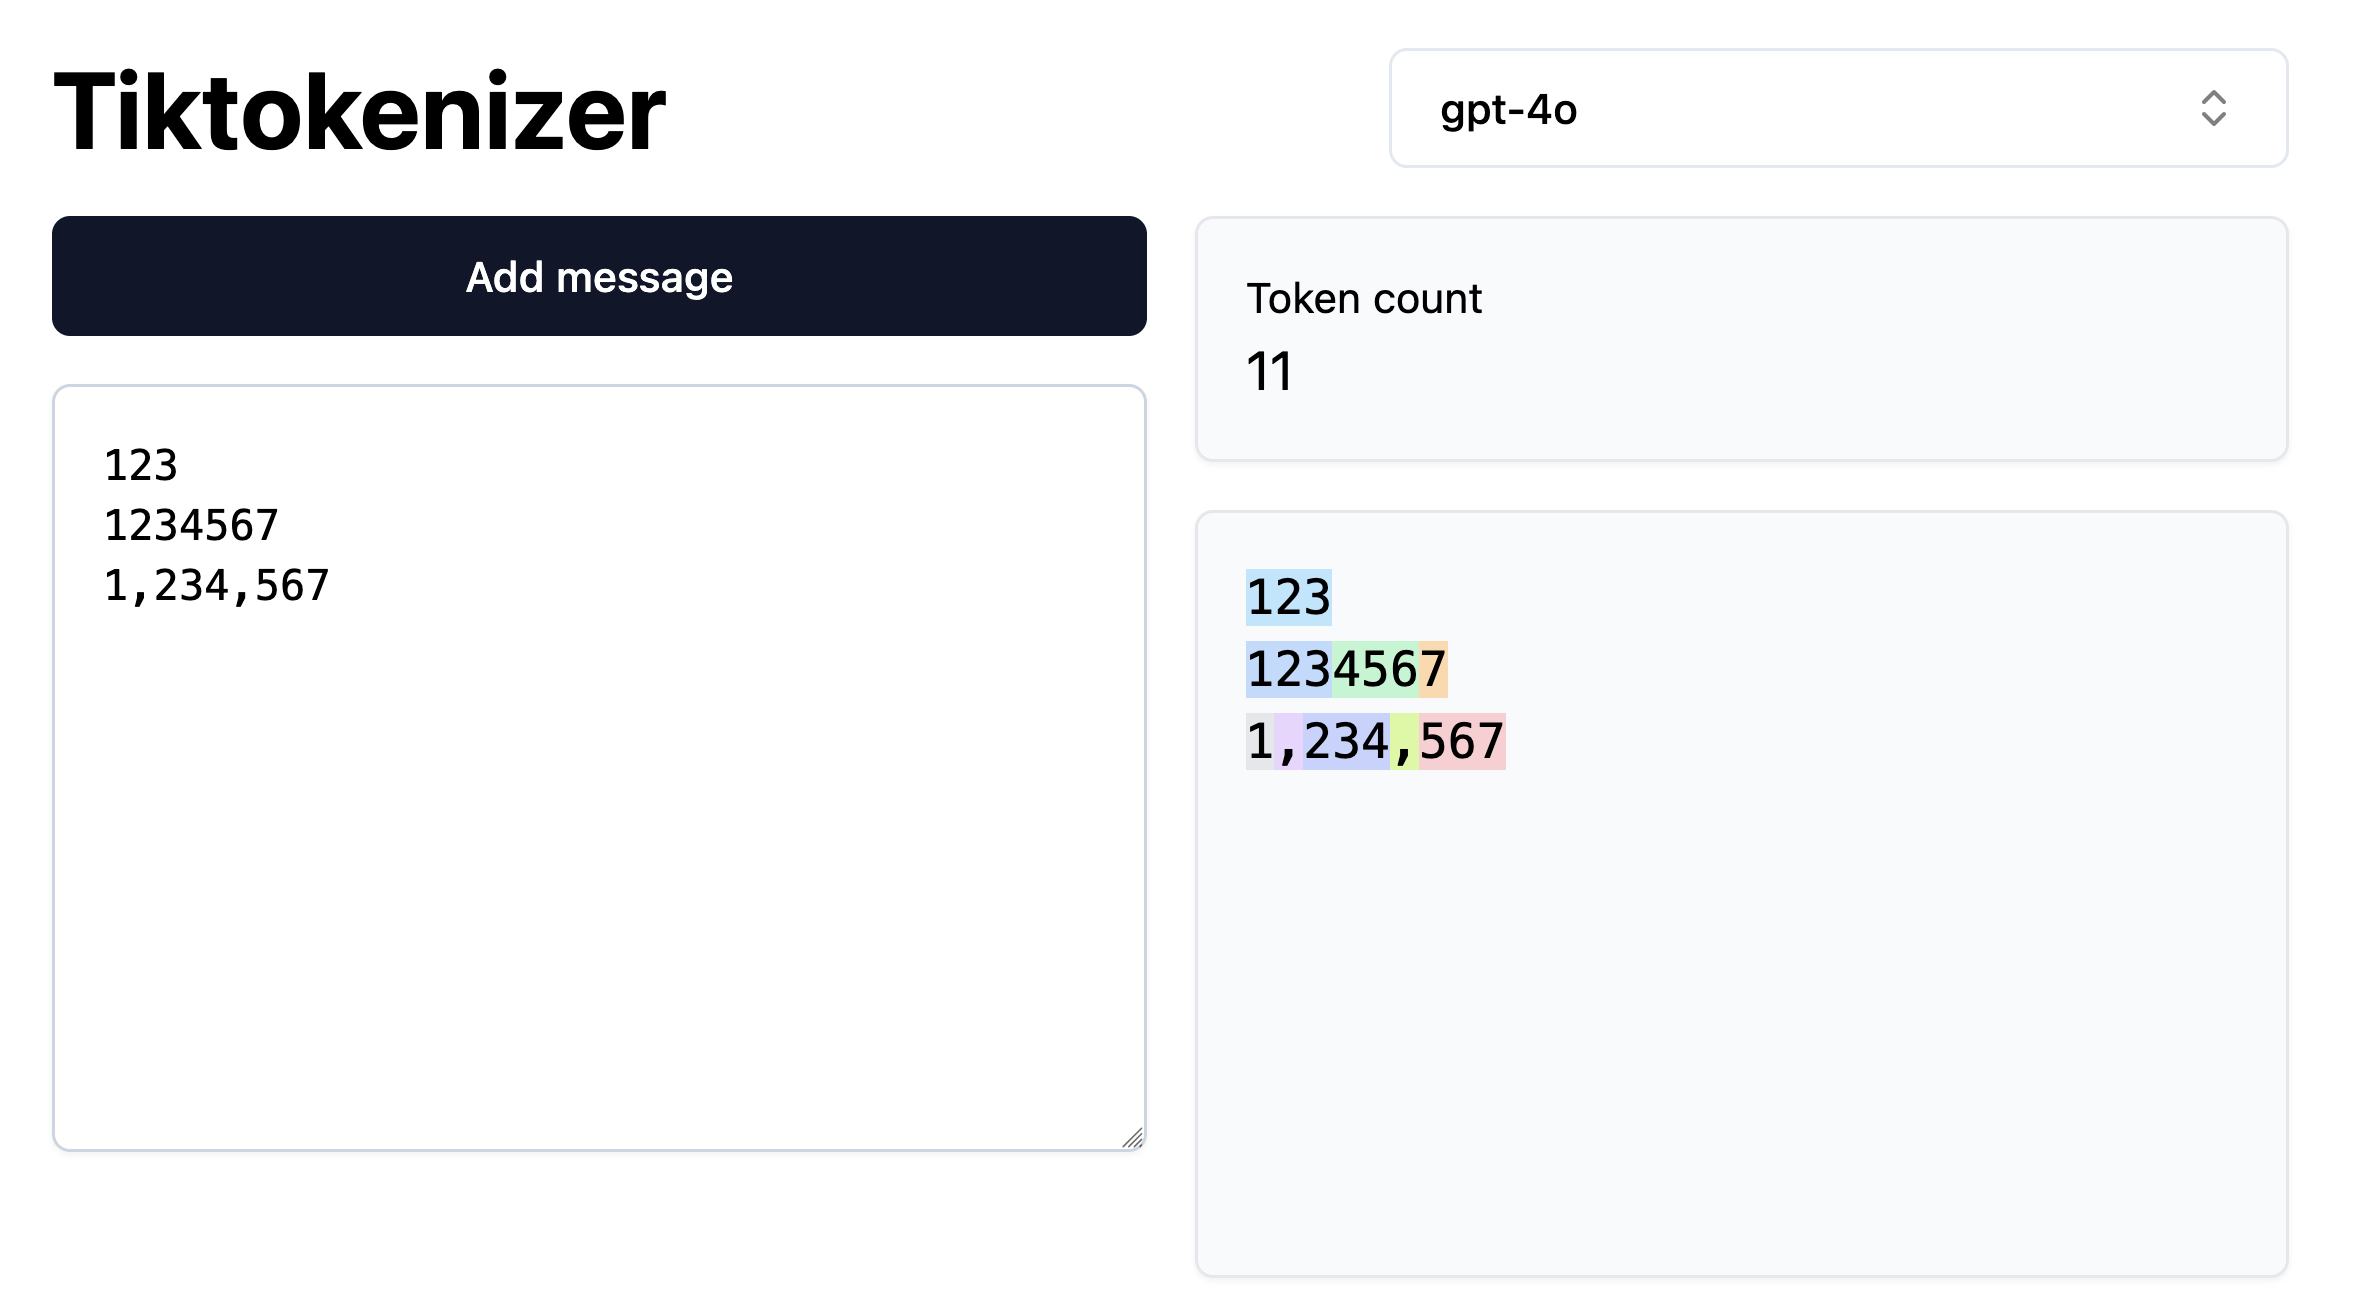
\includegraphics[keepaspectratio]{res/gpt4o-tokenization.png}}
\caption{GPT-4o tokenization of different numerical quantities,
displaying the L2R clustering and the comma trick to force R2L
clustering.}
\end{figure}

This could be happening for different reasons, for example:

\begin{itemize}
\item
  Arithmetic operations would still work locally in the 0-999 range,
  which allows for a correct reading on them and possible generalization
  on a larger scale, which counteracts the unintuitive clustering
  scheme.
\item
  The forced tokenization also happens in the data, as numbers are often
  separated by punctuation in clusters of 3 digits, right to left, for
  legibility reasons (\citeproc{ref-singh2024}{Singh \& Strouse, 2024}).
\item
  There's a geometric bias towards the right mode of operation given by
  the structures that form in the space to compute mathematical
  operations. This is the hypothesis that will be explored.
\end{itemize}

At the very least, the data being biased towards a R2L representation
(in the form of using the Arabic number system and adopting legibility
rules that accommodate right to left calculations) leads to embeddings
that maintain that bias even when learned in a L2R fashion. This can be
a possible hint towards the optimality of certain representations
compared to others, given the resilience in preferring a certain
tokenization scheme over the one the model is trained on.

\begin{longtable}[]{@{}ll@{}}
\toprule\noalign{}
\textbf{Model} & \textbf{Strategy} \\
\midrule\noalign{}
\endhead
\bottomrule\noalign{}
\tabularnewline
\caption{Language models with their respective tokenization strategy for
numbers.}
\endlastfoot
LLaMA 1 \& 2 & Single digit \\
LLaMA 3 & L2R chunks of 3 digits \\
OLMo 2 & L2R chunks of 3 digits \\
GPT-2 & Pure BPE \\
GPT-3.5 / GPT-4 & L2R chunks of 3 digits \\
Claude 3 / Claude 4 & R2L chunks of 3 digits \\
\end{longtable}

\clearpage

\section{Strategies for mathematical improvements through
embeddings}\label{strategies-for-mathematical-improvements-through-embeddings}

Beyond improving tokenization, there have been other, more comprehensive
approaches to the improvement of the representation of numeric values.
xVal is a notable one, as its approach encompasses real numbers beyond
just integers and does away with learning different representation for
each number.

The idea is maximizing the inductive bias in the representation by
having embeddings that are computed based on the number to be
represented (\citeproc{ref-golkar2023}{Golkar et al., 2023}). Numerical
values represented by a single embedding vector associated with the
\texttt{{[}NUM{]}} special token, that gets scaled on the basis of the
numerical value to represent. There is an assumption made so that this
works: the semantics of magnitude work as they pass from the represented
object to the structure of the representation.

This fits very well with the idea of reification, which will be
described later (\citeproc{ref-murray2010}{Murray, 2010}): the
embedding, beyond its qualities as representational object, becomes an
entity with features that actively aid in the calculation process.

The model uses two separate heads for number and token predictions. If
the token head predicts a \texttt{{[}NUM{]}} token as the successor, the
number head gets activated and outputs a scalar. The rest of the weights
in the transformer blocks are shared, allowing the learning of
representations that are useful for both discrete text prediction and
continuous numerical prediction. This means the model develops
number-aware internal representations throughout all its layers, not
just at the output. The shared weights force the model to learn features
that work for both linguistic and mathematical reasoning simultaneously.

The approach is shown to improve performance over a series of other
techniques, mostly using a standard notation to represent numbers
(\citeproc{ref-golkar2023}{Golkar et al., 2023}). This very thesis has
been inspired by the xVal paper, with one of its initial goals being to
find good representations for computed numerical embeddings.

There are several different approaches to improving math performance in
LLMs that don't necessarily come directly from training, but from a
better understanding of how representations work. Other approaches
include giving models better positional information about digits within
numbers, such as Abacus Embeddings (\citeproc{ref-mcleish2024}{McLeish
et al., 2024}), which encode each digit's position relative to the start
of the number and can improve arithmetic performance substantially.

While on one hand particular modes of numerical cognition can be
explored through explicitly reifying the representation (through the
xVal approach), what the rest of the analysis hinges on is whether LLMs
develop such structures on their own, by looking at their embeddings, as
this could hypothetically inform us on how to build these structures
ourselves in a more direct way than training.

\section{Savant syndrome and spatial
representations}\label{savant-syndrome-and-spatial-representations}

Savant syndrome is a rare condition in which people show exceptional
proclivity towards certain specific activities, usually accompanied by
great impairments in other areas of their lives. Savants can have
exceptional abilities in math, art, music and other fields, as well as
instant calculation abilities that don't seem to come through
algorithmic processing.

A case study of a Savant patient DT (\citeproc{ref-murray2010}{Murray,
2010}) reveals a mathematical cognitive architecture with the following
characteristics:

\begin{itemize}
\tightlist
\item
  has sequence-space synesthesia with a ``mathematical landscape''
  containing numbers 0-9999
\item
  each number possesses specific colors, textures, sizes, and sometimes
  movements or sounds
\item
  prime numbers have distinctive object properties that distinguish them
  from other numbers
\item
  arithmetic calculations happen automatically
\item
  solutions appear as part of his visual landscape without conscious
  effort
\item
  fMRI studies showed that even unstructured number sequences had
  coherent visual structure for DT.
\end{itemize}

Murray argues that savants possess highly accessible concrete
representations of abstract concepts, for which she uses the term
reification - the conversion of abstract concepts into concrete, spatial
entities that can be directly ``inspected'' rather than computed.

Sequence-space synesthesia is the spontaneous visualization of numerical
sequences in organized spatial arrangements. The remarkable mathematical
abilities of savants with this condition suggest that their specialized
perceptual representations confer significant computational advantages
over normal human numerical calculation abilities.

Given that the spatial arrangement confers advantages in numerical
calculation to the subject, we can pose the question: are there specific
spatial arrangements that enable advantageous numerical calculations,
and are those present or replicable in LLMs? The spatial idea is easily
translatable from the perceptive sphere to the representational one, by
considering LLM embeddings. If these come through because of geometric
properties of the structures, and going with the assumption that those
structures are replicable in the high-dimensional vector spaces we're
working with, it would follow that strict optimization through gradient
descent could be a possible way to make them come about.

\section{The Platonic Representation
Hypothesis}\label{the-platonic-representation-hypothesis}

According to (\citeproc{ref-huh2024}{Huh et al., 2024}) AI models,
particularly deep networks, are converging. The central hypothesis is
that different models are converging toward a shared statistical model
of reality, akin to Plato's concept of an ideal reality. This
representation is termed the Platonic representation.

This convergence appears to be driven by several selective pressures:
larger models have more capacity to find optimal representations; models
trained on more diverse tasks are constrained to find solutions that
work across multiple domains; and deep networks have implicit biases
toward simpler solutions.

For the investigation of numerical representations, this suggests that
if there are indeed optimal geometric structures for mathematical
reasoning, different models might naturally converge toward them during
training. The shape suggested (the helix) has properties on an
information-theory basis that make its use as a learning geometry more
likely (\citeproc{ref-kantamneni2025}{Kantamneni \& Tegmark, 2025}). In
particular, their self-similarity can be a useful error-correcting
property.

\section{The Helix and its role in LLM
addition}\label{the-helix-and-its-role-in-llm-addition}

During the final process of literature review of this thesis, a paper
was found that recontextualized some of the findings seen here.
(\citeproc{ref-kantamneni2025}{Kantamneni \& Tegmark, 2025}) has
revealed how mid-sized language models including GPT-J, Pythia-6.9B, and
Llama3.1-8B employ a helix to encode and manipulate numerical values
during arithmetic operations. The helix gets fit with the operands
required, and through structural manipulation via the ``Clock
algorithm'' performs addition by rotating helical representations and
reading out the final answer. From an information-theoretic perspective,
the authors demonstrate that helical representations provide significant
computational advantages over linear encodings, offering built-in
redundancy and error-correction properties. Even with highly precise
linear representations (\(R^2 = 0.997\)), linear addition achieves less
than 20\% accuracy while the helical approach achieves over 80\%,
suggesting the periodic structure serves as an error-correcting
mechanism analogous to how humans use decimal digits rather than slide
rules for precise calculation.

In looking at the numerical embeddings of OLMo and Llama models, we
observe very similar structures as the ones described in the paper,
which gives more comprehensive explanations on how the structures are
employed to perform mathematical operations such as addition, done from
a mechanistic interpretability perspective. MI attempts to explain the
model workings through the reverse engineering of it, and going through
the motions of the network. The work presented here will limit itself to
graphical visualization of single-token embeddings and feature analysis,
although the perspective presented by Kantamneni et al certainly seems
to give partial confirmation to the findings here presented.

\clearpage

\section{Dimensionality reduction and Embedding
Visualization}\label{dimensionality-reduction-and-embedding-visualization}

To visualize and analyze the high-dimensional embedding spaces that LLMs
use for numerical representations, we need techniques that make the
underlying structure evident. For this reason, we employ the following
dimensionality reduction techniques:

\begin{itemize}
\item
  \textbf{SVD (Singular Value Decomposition)} is a fundamental matrix
  factorization that decomposes any matrix \(A\) into three component
  matrices: \(A = U\Sigma V^T\), where \(U\) and \(V\) contain
  orthogonal vectors (left and right singular vectors respectively) and
  \(\Sigma\) contains the singular values on its diagonal. SVD reveals
  the underlying structure of the matrix by identifying the principal
  directions of variation and their relative importance through the
  singular values.
\item
  \textbf{PCA (Principal Component Analysis)} emerges as a specific
  application of SVD. By applying SVD to a centered data matrix (where
  each variable has been mean-centered), the right singular vectors
  \(V\) become the principal components - the directions of maximum
  variance in the data. The singular values in \(\Sigma\) are directly
  related to the eigenvalues of the covariance matrix.
\item
  \textbf{t-SNE (t-Distributed Stochastic Neighbor Embedding)}
  (\citeproc{ref-maaten2008}{Maaten \& Hinton, 2008}) converts
  similarities between data points in high-dimensional space into
  probabilities, then uses gradient descent to minimize the divergence
  between these probabilities and those of points in a low-dimensional
  embedding. It excels at preserving local neighborhood structure,
  making clusters very distinct in the visualization. However, t-SNE can
  distort global structure and distances between distant clusters become
  less meaningful, making it primarily useful for identifying local
  groupings in numerical embeddings.
\item
  \textbf{UMAP (Uniform Manifold Approximation and Projection)}
  (\citeproc{ref-mcinnes2020}{McInnes et al., 2020}) also preserves
  local structure like t-SNE, but additionally maintains more of the
  global structure through its foundation in topological data analysis.
  UMAP constructs a topological representation of the data in high
  dimensions, then uses stochastic gradient descent to optimize a
  low-dimensional representation to have similar topological properties.
  This makes it better suited for analyzing how models organize
  numerical concepts across different scales - both local clusters of
  similar numbers and global relationships between distant numerical
  regions.
\end{itemize}

\chapter{Implementation}\label{implementation}

The aim of the project was the realization of a framework to enable the
analysis and visualization of embeddings. To achieve this, we used three
parts:

\begin{itemize}
\item
  an extraction and sampling layer, used to load models from HuggingFace
  and extracting the parts of the embeddings layer of interest for this
  inquiry.
\item
  a storage layer, meant to store the selected samples in an easy to
  retrieve manner. In particular, during the course of this project we
  focused on sampling integers and some random embeddings, to have a
  comparison to see whether the structures formed were artifacts of the
  dimensionality reduction technique used.
\item
  a CLI, to provide a user interface for the download, extraction and
  sampling of embeddings from HuggingFace models
\item
  an analyzer, meant to compute base statistics about the embeddings and
  to extract results from the PCA analysis and give insights on various
  properties of the embeddings, such as explained variance of the
  various dimensions (through PCA) and correlation between numerical
  sequences and features.
\item
  a visualizer, to create plots that give a visual intuition of the
  structures underneath the embedding data.
\item
  a dashboard to display interactive visualization and to provide
  interactive data analysis features.
\end{itemize}

The following libraries have been employed in the making of this
project:

\begin{itemize}
\tightlist
\item
  \texttt{typer} for implementing the CLI
\item
  \texttt{transformers} and \texttt{torch} for model download and
  embeddings extraction
\item
  \texttt{numpy}, \texttt{pandas}, \texttt{sklearn}, \texttt{sympy} and
  \texttt{umap} for math and calculation purposes
\item
  \texttt{altair} and \texttt{plotly} for 2D and 3D plotting
  respectively
\item
  \texttt{marimo} for notebook and reactive dashboard functionality
\end{itemize}

\clearpage

\section{Storage layer}\label{storage-layer}

The storage layer allows storing embeddings samples from any HuggingFace
model without loading the whole model, as doing so was very often
impractically slow as a lot of the work was done in a
resource-constrained environment.

The sample data was stored in instances of the \texttt{EmbeddingsSample}
class (lst.~\ref{lst:embeddingsample}), along with metadata reporting
the source model ID and, for random samples, the seed used for
replicability purposes.

\begin{codelisting}

\caption{Container classes for embeddings samples and their
metadata.}\label{lst:embeddingsample}

\begin{Shaded}
\begin{Highlighting}[]

\AttributeTok{@dataclass}
\KeywordTok{class}\NormalTok{ IntegerSampleMeta:}
\NormalTok{    model\_id: }\BuiltInTok{str}
\NormalTok{    tag: Literal[}\StringTok{"integers"}\NormalTok{] }\OperatorTok{=} \StringTok{"integers"}

\AttributeTok{@dataclass}
\KeywordTok{class}\NormalTok{ RandomSampleMeta:}
\NormalTok{model\_id: }\BuiltInTok{str}
\NormalTok{    sample\_size: }\BuiltInTok{int}
\NormalTok{    seed: }\BuiltInTok{int}
\NormalTok{    tag: Literal[}\StringTok{"random"}\NormalTok{] }\OperatorTok{=} \StringTok{"random"}

\AttributeTok{@dataclass}
\KeywordTok{class}\NormalTok{ ReducedSampleMeta:}
\NormalTok{    original: EmbeddingsSampleMeta}
\NormalTok{    estimator: BaseEstimator}
\NormalTok{    tag: Literal[}\StringTok{"reduced"}\NormalTok{] }\OperatorTok{=} \StringTok{"reduced"}

\AttributeTok{@dataclass}
\KeywordTok{class}\NormalTok{ EmbeddingsSample[M: EmbeddingsSampleMeta]:}
\NormalTok{    sample\_id: }\BuiltInTok{int}
\NormalTok{    meta: M}
\NormalTok{    embeddings\_df: pd.DataFrame }\OperatorTok{=}\NormalTok{ field(}\BuiltInTok{repr}\OperatorTok{=}\VariableTok{False}\NormalTok{)}
\end{Highlighting}
\end{Shaded}

\end{codelisting}

Initially, the storage of each sample was done in a dedicated Parquet
file, an efficient file format that would have provided easy
serialization of Pandas dataframes, which were the main data structure
employed in the analysis. While initially adequate, this implementation
didn't allow for easy sample metadata storage, and required an ad-hoc
cataloguing system based on filesystem names to store and retrieve items
on the basis of their metadata.

To address this, a choice was made to implement a more proper storage
layer. It was realized using DuckDB, a single-file database similar to
SQLite that provides vector functionality appropriate for the storage of
embeddings. DuckDB also offers facilities to work directly on dataframes
using SQL queries, and exchanging data between dataframes and the
database in this way, which revealed very useful for loading purposes.

\begin{codelisting}

\caption{SQL schema for the storage layer.}\label{lst:sqlschema}

\begin{Shaded}
\begin{Highlighting}[]
\KeywordTok{CREATE} \KeywordTok{OR} \KeywordTok{REPLACE} \KeywordTok{TABLE}\NormalTok{ embeddings (}
\NormalTok{    model\_id }\DataTypeTok{VARCHAR} \KeywordTok{NOT} \KeywordTok{NULL}\NormalTok{,}
\NormalTok{    token\_id }\DataTypeTok{INTEGER} \KeywordTok{NOT} \KeywordTok{NULL}\NormalTok{,}
\NormalTok{    token }\DataTypeTok{VARCHAR} \KeywordTok{NOT} \KeywordTok{NULL}\NormalTok{,}
\NormalTok{    embeddings }\DataTypeTok{FLOAT}\NormalTok{[] }\KeywordTok{NOT} \KeywordTok{NULL}\NormalTok{,}
    \KeywordTok{PRIMARY} \KeywordTok{KEY}\NormalTok{ (model\_id, token\_id),}
\NormalTok{);}

\KeywordTok{CREATE} \KeywordTok{OR} \KeywordTok{REPLACE} \KeywordTok{SEQUENCE}\NormalTok{ embedding\_id\_seq;}
\KeywordTok{CREATE} \KeywordTok{OR} \KeywordTok{REPLACE} \KeywordTok{TABLE}\NormalTok{ samples (}
\NormalTok{    sample\_id }\DataTypeTok{INTEGER} \KeywordTok{DEFAULT}\NormalTok{ NEXTVAL(}\StringTok{\textquotesingle{}embedding\_id\_seq\textquotesingle{}}\NormalTok{) }\KeywordTok{PRIMARY} \KeywordTok{KEY}\NormalTok{,}
\NormalTok{    model\_id }\DataTypeTok{VARCHAR} \KeywordTok{NOT} \KeywordTok{NULL}\NormalTok{,}
\NormalTok{    meta JSON,}
\NormalTok{    created\_at }\DataTypeTok{TIMESTAMP} \KeywordTok{DEFAULT} \FunctionTok{CURRENT\_TIMESTAMP}\NormalTok{,}
\NormalTok{);}

\KeywordTok{CREATE} \KeywordTok{OR} \KeywordTok{REPLACE} \KeywordTok{TABLE}\NormalTok{ embedding\_to\_sample (}
\NormalTok{    model\_id }\DataTypeTok{VARCHAR} \KeywordTok{NOT} \KeywordTok{NULL}\NormalTok{,}
\NormalTok{    token\_id }\DataTypeTok{INTEGER} \KeywordTok{NOT} \KeywordTok{NULL}\NormalTok{,}
\NormalTok{    sample\_id }\DataTypeTok{INTEGER} \KeywordTok{NOT} \KeywordTok{NULL}\NormalTok{,}
    \KeywordTok{PRIMARY} \KeywordTok{KEY}\NormalTok{ (model\_id, token\_id, sample\_id),}
\NormalTok{);}
\end{Highlighting}
\end{Shaded}

\end{codelisting}

\clearpage

\section{Extraction and Sampling}\label{extraction-and-sampling}

Extraction is performed by downloading models using HuggingFace's
Transformers library, which allows for download and deployment of
popular open source models.

\begin{codelisting}

\caption{Extraction class for embeddings}\label{lst:extractor}

\begin{Shaded}
\begin{Highlighting}[]
\KeywordTok{class}\NormalTok{ HFEmbeddingsExtractor:}
    \CommentTok{"""Extracts embeddings from a Hugging Face model."""}

    \KeywordTok{def} \FunctionTok{\_\_init\_\_}\NormalTok{(}\VariableTok{self}\NormalTok{, name\_or\_path: }\BuiltInTok{str}\NormalTok{):}
        \VariableTok{self}\NormalTok{.name\_or\_path }\OperatorTok{=}\NormalTok{ name\_or\_path}

    \AttributeTok{@cached\_property}
    \KeywordTok{def}\NormalTok{ embeddings(}\VariableTok{self}\NormalTok{):}
\NormalTok{        model }\OperatorTok{=}\NormalTok{ AutoModel.from\_pretrained(}\VariableTok{self}\NormalTok{.name\_or\_path)}
\NormalTok{        model.}\BuiltInTok{eval}\NormalTok{()}
\NormalTok{        embeddings }\OperatorTok{=}\NormalTok{ model.embed\_tokens}
        \ControlFlowTok{return}\NormalTok{ embeddings}

    \KeywordTok{def}\NormalTok{ extract(}\VariableTok{self}\NormalTok{, token\_ids):}
        \ControlFlowTok{with}\NormalTok{ torch.no\_grad():}
\NormalTok{            token\_ids }\OperatorTok{=}\NormalTok{ torch.tensor(token\_ids)}
            \ControlFlowTok{return} \VariableTok{self}\NormalTok{.embeddings.forward(token\_ids).squeeze().numpy()}
\end{Highlighting}
\end{Shaded}

\end{codelisting}

LLMs that make use of a tokenization step receive their sentences in
input as a list of token IDs, where each token ID corresponds to an
embedding vector. It is the LLM's tokenizer responsibility to take
sentences, split them at the appropriate token boundary, adding special
tokens where necessary, and convert them into token IDs for the LLM
processing.

The logic to do this is split between the \texttt{HFTokenizerWrapper}
(lst.~\ref{lst:tokenizer}) and \texttt{HFEmbeddingsSampler}
(lst.~\ref{lst:sampler}) classes. \texttt{HFTokenizerWrapper} invokes
the tokenizer to get the token IDs that correspond to the embeddings of
interest (avoiding special tokens, like
\texttt{\textless{}Beginning\ of\ Sentence\textgreater{}} and such),
while \texttt{HFEmbeddingsSampler} has the logic for integer and random
selection.

\begin{codelisting}

\caption{HFTokenizerWrapper class, providing utility functions for
tokenization.}\label{lst:tokenizer}

\begin{Shaded}
\begin{Highlighting}[]
\KeywordTok{class}\NormalTok{ HFTokenizerWrapper:}
    \CommentTok{"""Wrapper for Hugging Face tokenizers."""}

    \KeywordTok{def} \FunctionTok{\_\_init\_\_}\NormalTok{(}\VariableTok{self}\NormalTok{, tokenizer):}
        \VariableTok{self}\NormalTok{.tokenizer }\OperatorTok{=}\NormalTok{ tokenizer}

    \KeywordTok{def}\NormalTok{ tokenize(}\VariableTok{self}\NormalTok{, tokens) }\OperatorTok{{-}\textgreater{}}\NormalTok{ torch.Tensor:}
        \ControlFlowTok{return} \VariableTok{self}\NormalTok{.tokenizer(}
\NormalTok{            tokens,}
\NormalTok{            add\_special\_tokens}\OperatorTok{=}\VariableTok{False}\NormalTok{,}
\NormalTok{            return\_attention\_mask}\OperatorTok{=}\VariableTok{False}\NormalTok{,}
\NormalTok{            return\_tensors}\OperatorTok{=}\StringTok{"pt"}\NormalTok{,}
\NormalTok{        )[}\StringTok{"input\_ids"}\NormalTok{]}

    \AttributeTok{@classmethod}
    \KeywordTok{def}\NormalTok{ from\_pretrained(cls, model\_id):}
\NormalTok{        tokenizer }\OperatorTok{=}\NormalTok{ AutoTokenizer.from\_pretrained(model\_id)}
        \ControlFlowTok{return}\NormalTok{ cls(tokenizer)}

    \KeywordTok{def}\NormalTok{ token\_ids\_to\_tokens(}\VariableTok{self}\NormalTok{, token\_ids):}
\NormalTok{        tokens }\OperatorTok{=} \VariableTok{self}\NormalTok{.tokenizer.convert\_ids\_to\_tokens(token\_ids)}
        \ControlFlowTok{return}\NormalTok{ [token }\ControlFlowTok{if}\NormalTok{ token }\KeywordTok{is} \KeywordTok{not} \VariableTok{None} \ControlFlowTok{else} \StringTok{"\textless{}unk\textgreater{}"} \ControlFlowTok{for}\NormalTok{ token }\KeywordTok{in}\NormalTok{ tokens]}
\end{Highlighting}
\end{Shaded}

\end{codelisting}

The sampling happens by first picking the tokens of interest. For
numbers, we first verify that the model uses a tokenization scheme
useful for the numeric analysis intended, by trying to tokenize each
integer from 0 onwards, up to a maximum ceiling of 10.000, until we find
the first integer that gets tokenized using more than one token. The
analysis is limited in scope to single-token integers in the range
0-999, as these parameters correspond to a multitude of open source
models available as of today. For random sampling, token IDs are picked
by doing a random extraction of numbers between 0 and the vocabulary
size of the model, and then proceeding similarly.

After the sampling process is completed, the results are returned as a
dataframe, along with the corresponding provenance metadata.

\begin{codelisting}

\caption{Code for \texttt{HFEmbeddingSampler}}\label{lst:sampler}

\begin{Shaded}
\begin{Highlighting}[]
\KeywordTok{class}\NormalTok{ HFEmbeddingsSampler:}
    \KeywordTok{def}\NormalTok{ \_single\_token\_integer\_ids(}\VariableTok{self}\NormalTok{, max\_value}\OperatorTok{=}\DecValTok{10\_000}\NormalTok{) }\OperatorTok{{-}\textgreater{}}\NormalTok{ Iterable[}\BuiltInTok{int}\NormalTok{]:}
        \ControlFlowTok{for}\NormalTok{ num }\KeywordTok{in} \BuiltInTok{range}\NormalTok{(max\_value):}
\NormalTok{            token\_ids }\OperatorTok{=} \VariableTok{self}\NormalTok{.tokenizer.tokenize(}\BuiltInTok{str}\NormalTok{(num)).squeeze()}
            \ControlFlowTok{if}\NormalTok{ token\_ids.ndim }\OperatorTok{==} \DecValTok{0}\NormalTok{:}
                \ControlFlowTok{yield}\NormalTok{ token\_ids.item()}
            \ControlFlowTok{else}\NormalTok{:}
                \ControlFlowTok{return}
\NormalTok{        warnings.warn(}
            \SpecialStringTok{f"All integers from 0 to max\_value=}\SpecialCharTok{\{}\NormalTok{max\_value}\SpecialCharTok{\}}\SpecialStringTok{ are single token. "}
            \StringTok{"There may be more single{-}token integers."}
\NormalTok{        )}

    \KeywordTok{def}\NormalTok{ single\_token\_integers(}\VariableTok{self}\NormalTok{) }\OperatorTok{{-}\textgreater{}} \BuiltInTok{tuple}\NormalTok{[pd.DataFrame, IntegerSampleMeta]:}
\NormalTok{        token\_ids }\OperatorTok{=}\NormalTok{ np.fromiter(}\VariableTok{self}\NormalTok{.\_single\_token\_integer\_ids(), }\BuiltInTok{int}\NormalTok{)}
\NormalTok{        tokens }\OperatorTok{=} \BuiltInTok{range}\NormalTok{(}\BuiltInTok{len}\NormalTok{(token\_ids))}
\NormalTok{        embeddings }\OperatorTok{=} \VariableTok{self}\NormalTok{.extractor.extract(token\_ids)}

\NormalTok{        df }\OperatorTok{=}\NormalTok{ make\_embeddings\_df(token\_ids, tokens, embeddings)}
\NormalTok{        meta }\OperatorTok{=}\NormalTok{ IntegerSampleMeta(model\_id}\OperatorTok{=}\VariableTok{self}\NormalTok{.model\_id)}

        \ControlFlowTok{return}\NormalTok{ df, meta}

\NormalTok{    ...}
    \KeywordTok{def}\NormalTok{ \_random\_token\_ids(}\VariableTok{self}\NormalTok{, sample\_size, seed):}
\NormalTok{        rng }\OperatorTok{=}\NormalTok{ np.random.default\_rng(seed)}
        \ControlFlowTok{return}\NormalTok{ rng.choice(}\VariableTok{self}\NormalTok{.tokenizer.vocab\_size, size}\OperatorTok{=}\NormalTok{sample\_size, replace}\OperatorTok{=}\VariableTok{False}\NormalTok{)}
\NormalTok{    ...}
\end{Highlighting}
\end{Shaded}

\end{codelisting}

\clearpage

\section{Analysis}\label{analysis}

Most of the analysis in done in the \texttt{EmbeddingsAnalyzer}
(lst.~\ref{lst:embeddingsanalyzer}) class, which reorganizes data and
provides it in a format suitable for consultation and visualization.

\begin{codelisting}

\caption{Initializing code for
\texttt{EmbeddingsAnalyzer}}\label{lst:embeddingsanalyzer}

\begin{Shaded}
\begin{Highlighting}[]
\AttributeTok{@dataclass}
\KeywordTok{class}\NormalTok{ EmbeddingsAnalyzer:}
\NormalTok{    embeddings\_df: pd.DataFrame}
\NormalTok{    meta: EmbeddingsSampleMeta}

    \AttributeTok{@classmethod}
    \KeywordTok{def}\NormalTok{ from\_sample(cls, sample: EmbeddingsSample):}
        \CommentTok{"""Initialize from an EmbeddingsSample."""}
        \ControlFlowTok{return}\NormalTok{ cls(}
\NormalTok{            embeddings\_df}\OperatorTok{=}\NormalTok{wide\_embeddings\_df(sample.embeddings\_df),}
\NormalTok{            meta}\OperatorTok{=}\NormalTok{sample.meta,}
\NormalTok{        )}
\end{Highlighting}
\end{Shaded}

\end{codelisting}

The format used for the embeddings here is a dataframe with the columns
\texttt{token}, \texttt{token\_id} and the embeddings spread out in
columns named \texttt{embeddings\_\{dimension\ index\}}. Even though
it's a little unwieldy, this allows for compatibility with most of the
libraries operating with dataframe that assume mono-dimensional column
indices with string column names. This class also provides the facility
for dimensional reduction through the \texttt{run\_estimator} method,
which takes an estimator as input and returns a new
\texttt{EmbeddingsAnalyzer} instance with the embeddings being fit
through the estimator.

A notable feature implemented here is the analysis of the correlations
between embedding features and mathematical sequences, done in the
\texttt{feature\_to\_sequence\_analysis\_df} method. This is done by
generating various mathematical sequences and then encoding them using
either:

\begin{itemize}
\tightlist
\item
  Direct encoding, for the ones that don't grow too much in value, like
  \(\log_n\) or \(n\). This simply means that the mathematical sequence
  vector the feature is tested against is produced by directly inserting
  the relative values, like \([log(0), log(1),
  log(2), \ldots]\)
\item
  One-hot encoding, for faster growing sequences. The indices that
  correspond to a value contained in sequence get the value 1, the
  others get the value 0.
\item
  Gaussian-smoothed one-hot encoding, where the values are passed
  through a Gaussian filter to check for smoother feature detection.
\end{itemize}

As a result of the analysis, a dataframe is produced that provides data
about features and their respective correlations.

\begin{codelisting}

\caption{Code for mathematical sequence
encoding.}\label{lst:mathencoding}

\begin{Shaded}
\begin{Highlighting}[]
\KeywordTok{def}\NormalTok{ one\_hot\_encode(sequence, size):}
    \ControlFlowTok{return}\NormalTok{ np.isin(np.arange(size), sequence).astype(}\BuiltInTok{int}\NormalTok{)}

\KeywordTok{def}\NormalTok{ one\_hot\_gaussian\_smooth(binary, sigma}\OperatorTok{=}\FloatTok{2.0}\NormalTok{):}
    \ControlFlowTok{return}\NormalTok{ gaussian\_filter1d(binary.astype(}\BuiltInTok{float}\NormalTok{), sigma}\OperatorTok{=}\NormalTok{sigma)}

\KeywordTok{def}\NormalTok{ make\_encoded\_sequences(max\_token: }\BuiltInTok{int}\NormalTok{, sigma: }\BuiltInTok{float} \OperatorTok{=} \FloatTok{2.0}\NormalTok{):}
\NormalTok{    encoded\_sequences }\OperatorTok{=}\NormalTok{ \{\}}

\NormalTok{    direct\_sequences }\OperatorTok{=}\NormalTok{ direct\_encoded\_base\_sequences(max\_token)}
    \ControlFlowTok{for}\NormalTok{ name, seq }\KeywordTok{in}\NormalTok{ direct\_sequences.items():}
\NormalTok{        encoded\_sequences[name, }\StringTok{"direct"}\NormalTok{] }\OperatorTok{=}\NormalTok{ seq}

\NormalTok{    binary\_sequences }\OperatorTok{=}\NormalTok{ binary\_encoded\_base\_sequences(max\_token)}
    \ControlFlowTok{for}\NormalTok{ name, seq }\KeywordTok{in}\NormalTok{ binary\_sequences.items():}
\NormalTok{        one\_hot }\OperatorTok{=}\NormalTok{ one\_hot\_encode(seq, max\_token)}
\NormalTok{        encoded\_sequences[name, }\StringTok{"binary"}\NormalTok{] }\OperatorTok{=}\NormalTok{ one\_hot}
\NormalTok{        encoded\_sequences[name, }\StringTok{"gauss"}\NormalTok{] }\OperatorTok{=}\NormalTok{ one\_hot\_gaussian\_smooth(one\_hot, sigma}\OperatorTok{=}\NormalTok{sigma)}

    \ControlFlowTok{return}\NormalTok{ encoded\_sequences}
\end{Highlighting}
\end{Shaded}

\end{codelisting}

\section{CLI}\label{cli}

The end user can make use of the tools by loading a model through the
CLI, which was programmed using the \texttt{typer} library. It can be
used to load model numerical and random samples into the database
through the command
\texttt{embcli\ load\ \textless{}hf\_model\_id\textgreater{}}, which can
then be listed and consulted through the Marimo dashboard.

\chapter{Embeddings Analysis}\label{embeddings-analysis}

\section{Methodology}\label{methodology}

The analytic part of this work consists in the search for structures in
LLM numerical embeddings. Two models are taken in consideration:

\begin{itemize}
\item
  OLMo-2-1124-7B (\citeproc{ref-olmo2025}{OLMo et al., 2025}) is a model
  by AllenAI, which is favorable to research uses thanks to the full
  disclosure of training data, code, logs and checkpoints. This model
  was trained on 4.05T tokens using a two-stage curriculum: initial
  pretraining on 3.90T tokens of web-based data, followed by a
  specialized mid-training phase on 150B high-quality tokens including
  10.7B synthetic mathematical data specifically designed to enhance
  numerical reasoning capabilities.
\item
  Llama-3.2-1B-Instruct (\citeproc{ref-grattafiori2024}{Grattafiori et
  al., 2024}), due to being a small and manageable model to do analysis
  with on limited hardware. This model derives from the Llama 3 family,
  which was trained on approximately 15T multilingual tokens with
  dynamic data mixing throughout training, including mathematical
  content integrated continuously rather than in separate phases.
\end{itemize}

Both models underwent single-pass training without data repetition,
meaning their numerical representations developed through one-time
exposure to mathematical content.

For each of these, dimensionality reduction is applied through PCA, SVD,
t-SNE and UMAP, and the results are used to produce 2D and 3D
visualization meant to show the geometric structure that the
representation assume in the space.

Then, an analysis of correlation with mathematical sequences is done:
for each dimension, we encode mathematically interesting sequences the
embedding features might be detecting for, and measure their Pearson
correlation coefficient along with their respective p-value. We adopt
the following encoding for sequences:

\begin{itemize}
\item
  direct, meaning we test the correlation directly with the sequence. We
  do this with plain integers in sequence (0, 1, 2, 3) and their
  logarithm (log(1), log(2), \ldots)
\item
  one hot encoded, for the sequences where the growth would be too fast
  to have meaningful detection through direct encoding. We tried this
  for Fibonacci, triangular, and prime numbers
\item
  Gaussian-smoothed one-hot encoded, same as last point but allowing a
  more gradual climb around the positions corresponding to the numbers
  by applying a Gaussian smoothing filter to the one-hot encoded vector.
\item
  Fourier encoding, as \(\sin\left(2 \pi  \cdot \frac{n_i}T\right)\) and
  \(\cos\left(2 \pi
  \cdot \frac{n_i}T\right)\) where \(n_i\) is the element of the
  sequence to be encoded and \(T \in \{1, 2, 5, 10, 100\}\) is a
  collection of possible periods of encoding, as suggested in
  (\citeproc{ref-kantamneni2025}{Kantamneni \& Tegmark, 2025}) as a
  possible way for features to encode numeric characteristics.
\end{itemize}

\clearpage

\section{OLMo-2-1124-7B}\label{olmo-2-1124-7b}

\subsection{Linear analysis}\label{linear-analysis}

\begin{figure}
\centering
\pandocbounded{\includesvg[keepaspectratio]{plots/OLMo-2-1124-7B_00_pca_components_gradient_v1.svg}}
\caption{Principal components 1 and 2 of the OLMo model. Random
embeddings sample for comparison.}\label{fig:olmo-pca}
\end{figure}

In fig.~\ref{fig:olmo-pca}, we plot the first two principal component of
the numerical embeddings, color-grading them on the basis of their
numerical value. The result shows that numerical tokens do not occupy
the embedding space randomly: they follow a constrained path that
preserves numerical relationships, suggesting that the model has learned
to encode ordering properties of the numbers within its representation.
The gradient is particularly smooth, suggesting that similar numbers
maintain spatial proximity in the reduced space. It's also notable that
in the top right of the curve, there seems to be a smaller curve
forming; it's better visible through the SVD visualizations, but that
part corresponds to single and double-digit integers replicating the
bigger overall structure of the lower curve.

\begin{figure}
\centering
\pandocbounded{\includesvg[keepaspectratio]{plots/OLMo-2-1124-7B_02_svd_components_gradient_v1.svg}}
\caption{SVD for the two main components of the OLMo model, with random
embeddings sample for comparison}\label{fig:olmo-svd}
\end{figure}

The relationship and similarities are even more clear in
fig.~\ref{fig:olmo-svd}, which, lacking the data centering done in the
PCA, shows a much more consistent geometric structure, showing that the
encoding of information likely happens in absolute distances rather than
just with relative positioning between data points. This will also
inform the strategies we use for reconstructing the datapoints with
UMAP, as we'll do projections that make use of Euclidean distance as
well as cosine similarity as a metric.

\begin{figure}
\centering
\includegraphics[width=0.5\linewidth,height=\textheight,keepaspectratio]{plots/olmo-svd-3d.png}
\caption{OLMo-2-1124-7B 3D visualization of SVD components
.}\label{fig:olmo-svd-3d}
\end{figure}

\begin{figure}
\centering
\pandocbounded{\includesvg[keepaspectratio]{plots/OLMo-2-1124-7B_03_svd_digit_visualizations_v1.svg}}
\caption{SVD coloring done by digit length and hundreds digit,
highlighting the clustering properties of the
embeddings.}\label{fig:olmo-svd-digits}
\end{figure}

Looking at fig.~\ref{fig:olmo-svd-digits}, the self-similar structure
repeating through different integer lengths is strinking. Models like
Qwen-2.5 do away with tokenizing numbers outside the single digits from
0 to 9, and this picture can offer a compelling explanation on why that
can be justified. In fact, it seems like the encoding of higher digit
quantities brings along a lot of redundancy. On the other hand, as
discussed for (\citeproc{ref-kantamneni2025}{Kantamneni \& Tegmark,
2025}), this same redundancy could be used by the models an error
correcting mechanism when it has to apply numerical operations, leading
to possibly better performance.

\subsubsection{Explained variance}\label{explained-variance}

\begin{figure}
\centering
\pandocbounded{\includesvg[keepaspectratio]{plots/OLMo-2-1124-7B_01_pca_variance_overview_v1.svg}}
\caption{OLMo PCA - explained variance
overview}\label{fig:olmo-variance}
\end{figure}

The explained variance by component plot (fig.~\ref{fig:olmo-variance},
left) shows a sharp drop within the first few components, meaning that
the first principal components capture dramatically more variance than
subsequent ones. The cumulative explained variance (right) shows that
approximatively 600 principal components are needed to reach 90\% of
explained variance.

By this we can conclude that the embeddings have a much lower intrinsic
dimensionality than their full 4096 dimensions, and that they lie on a
low-dimensional manifold in the full representation space. Only
one-fifth of the total embedding space is necessary to capture 90\% of
the variance, and, as described earlier, the structures already encoded
provide already a lot of redundancy.

\subsection{Non-linear analysis}\label{non-linear-analysis}

\begin{figure}
\centering
\pandocbounded{\includesvg[keepaspectratio]{plots/OLMo-2-1124-7B_07_tsne_components_gradient_v1.svg}}
\caption{t-SNE visualization for OLMo embeddings.}\label{fig:olmo-tsne}
\end{figure}

\begin{longtable}[]{@{}ll@{}}
\toprule\noalign{}
\textbf{Parameter} & \textbf{Value} \\
\midrule\noalign{}
\endhead
\bottomrule\noalign{}
\tabularnewline
\caption{\label{tbl:tsne-params}t-SNE hyperparameters for the presented
plots.}
\endlastfoot
perplexity & 75 \\
max\_iter & 3000 \\
learning\_rate & 50 \\
early\_exaggeration & 20 \\
random\_state & 42 \\
\end{longtable}

The t-SNE visualization in fig.~\ref{fig:olmo-tsne} shows a distinctive
branching pattern emanating from a central region, with low numbers at
the center and higher ones radiating outward. The color progression
follows these branches, indicating that numerical sequences are
preserved along each arm. The gradient seems also to transition
circularly; branches with gradually increasing numbers turn around the
center before abruptly getting back to the start. When interpreting the
colors as indicators of depth, it can look like a spiral from a top-down
perspective, giving a visual confirmation of what has been said about
helical structures in (\citeproc{ref-kantamneni2025}{Kantamneni \&
Tegmark, 2025}).

\begin{figure}
\centering
\pandocbounded{\includesvg[keepaspectratio]{plots/OLMo-2-1124-7B_09_umap_cosine_components_gradient_v1.svg}}
\caption{UMAP visualization with cosine
distance}\label{fig:olmo-umap-cosine}
\end{figure}

\begin{figure}
\centering
\pandocbounded{\includesvg[keepaspectratio]{plots/OLMo-2-1124-7B_11_umap_euclidean_components_gradient_v1.svg}}
\caption{UMAP visualization with Euclidean
distance}\label{fig:olmo-umap-euclidean}
\end{figure}

UMAP has been run using both Euclidean
(fig.~\ref{fig:olmo-umap-euclidean}) and cosine distances
(fig.~\ref{fig:olmo-umap-cosine}), since the SVD visualization has shown
that absolute distances can matter in this model. In the UMAP case we
can observe a loss of shape similar to what happened in the PCA and SVD
case. While the structure is congruent when using Euclidean distances,
segregated clusters form when representing cosine similarity, with their
predominant criterion of division being the hundreds' digit. Using
Euclidean distances gives a picture similar to t-SNE, but projected and
stretched and with more dispersion for numbers close to zero. The
spiral-like conformation is also notable here.

\subsection{Correlation with mathematical
properties}\label{correlation-with-mathematical-properties}

\begin{longtable}[]{@{}
  >{\raggedright\arraybackslash}p{(\linewidth - 8\tabcolsep) * \real{0.1579}}
  >{\raggedright\arraybackslash}p{(\linewidth - 8\tabcolsep) * \real{0.1579}}
  >{\raggedright\arraybackslash}p{(\linewidth - 8\tabcolsep) * \real{0.2982}}
  >{\raggedleft\arraybackslash}p{(\linewidth - 8\tabcolsep) * \real{0.1930}}
  >{\raggedleft\arraybackslash}p{(\linewidth - 8\tabcolsep) * \real{0.1930}}@{}}
\toprule\noalign{}
\begin{minipage}[b]{\linewidth}\raggedright
dimension
\end{minipage} & \begin{minipage}[b]{\linewidth}\raggedright
property
\end{minipage} & \begin{minipage}[b]{\linewidth}\raggedright
encoding
\end{minipage} & \begin{minipage}[b]{\linewidth}\raggedleft
correlation
\end{minipage} & \begin{minipage}[b]{\linewidth}\raggedleft
p\_value
\end{minipage} \\
\midrule\noalign{}
\endhead
\bottomrule\noalign{}
\tabularnewline
\caption{\label{tbl:olmo-correlations}Feature-sequence correlations in
OLMo-2.}
\endlastfoot
514 & log & direct & -0.67287 & 8.4465e-133 \\
3085 & even & direct & -0.60990 & 6.3840e-103 \\
3085 & numbers & direct & -0.60990 & 6.3840e-103 \\
3085 & log & direct & -0.60653 & 1.6467e-101 \\
514 & fibonacci & gauss & 0.37430 & 1.3043e-34 \\
2538 & fibonacci & gauss & 0.35112 & 2.1919e-30 \\
514 & primes & gauss & 0.26358 & 2.3511e-17 \\
695 & primes & fourier\_cos\_t10 & -0.22069 & 1.6980e-12 \\
2538 & fibonacci & fourier\_cos\_t5 & -0.18336 & 5.2002e-09 \\
\end{longtable}

A lot of features (tbl.~\ref{tbl:olmo-correlations},
fig.~\ref{fig:olmo-properties}) correlate very significatively with
magnitude, giving confirmation of the semantic connection between the
embedding value and the number represented. We find:

\begin{itemize}
\tightlist
\item
  Dimension 514 has a high correlation (0.37) with Fibonacci numbers
  using Gauss one-hot encoding, and with prime numbers with Gauss
  one-hot encoding (0.26).
\item
  There are other dimensions are also correlated with Fibonacci and
  Primes, to a lesser extent, and Fourier encoding seems to show weaker
  ties than one-hot Gaussian encoding.
\end{itemize}

Although while these can be useful clues about the relation between the
features and the numerical properties they're correlated with, they do
not explain by themselves how and why the features are tied to those
properties. The correlation with Fibonacci numbers in particular is high
enough to not resemble a pure coincidence, especially in such a
high-dimensional space. We can speculatively make some hypotheses:

\begin{itemize}
\tightlist
\item
  Features in the embedding might work as hierarchical detectors, with
  some of them being broad-scope, general detectors of numbers of
  interest (dimension 514), and others being more specific to certain
  properties (2538 to Fibonacci numbers).
\item
  The correlation with the features is tied with the geometry of the
  embedding space. The Fibonacci numbers have ties to spiral structures
  (in particular golden spirals), which may have a relation to the
  self-similar structures observed.
\end{itemize}

Further study would be needed to untangle the relationship between
mathematical sequences and features, although having a dimension (514)
with such a strong correlation with Fibonacci numbers and such a low
p-value doesn't seem dismissible over random chance.

\begin{figure}
\centering
\includesvg[width=0.45\linewidth,height=\textheight,keepaspectratio]{plots/OLMo-2-1124-7B_strong_property_correlations_v1.svg}
\caption{Mathematical sequences against the number of associated
strongly correlated embedding dimensions.}\label{fig:olmo-properties}
\end{figure}

\clearpage

\section{Llama-3.2-1B-Instruct}\label{llama-3.2-1b-instruct}

\subsection{Linear analysis}\label{linear-analysis-1}

\begin{figure}
\centering
\pandocbounded{\includesvg[keepaspectratio]{plots/Llama-3.2-1B-Instruct_pca_components_gradient_digit_length_v1.svg}}
\caption{PCA visualization of Llama embeddings.}\label{fig:llama-pca}
\end{figure}

The LLaMa PCA plot (fig.~\ref{fig:llama-pca}) shows a similar picture to
the OLMo one: a curve with smooth, gradual transitions between numeric
quantities. The self-similar, recursive structure based on digit count
is immediately visible in the PCA plot, as there is a much more striking
division and a separation between numbers of different digit size. It is
remarkable how the replication of the same structures for different
digit counts stays present in different models.

\begin{figure}
\centering
\pandocbounded{\includesvg[keepaspectratio]{plots/Llama-3.2-1B-Instruct_02_svd_components_gradient_v1.svg}}
\caption{SVD visualization of Llama embeddings compared to random
sample.}\label{fig:llama-svd}
\end{figure}

The SVD plot shows a linear arrangement - numbers form an almost
straight diagonal line from small to large values. However, this
apparently linear picture changes drastically once we also take into
account the third component, showing a much more tridimensional picture,
looking like the curves observed in PCA after a diagonal rotation. The
3D projection (fig.~\ref{fig:llama-svd-3d}) really shines here, showing
how the same structure is repeating at different distances and angles of
rotation.

\begin{figure}
\centering
\pandocbounded{\includesvg[keepaspectratio]{plots/Llama-3.2-1B-Instruct_svd_components_gradient_0-2_v1.svg}}
\caption{Llama SVD visualizations of first and third
component.}\label{fig:llama-svd-digits}
\end{figure}

\begin{figure}
\centering
\pandocbounded{\includegraphics[keepaspectratio]{plots/llama_svd_3d.png}}
\caption{3D projection of LLaMa 3.2 embeddings after
SVD}\label{fig:llama-svd-3d}
\end{figure}

\subsubsection{Explained variance}\label{explained-variance-1}

\begin{figure}
\centering
\pandocbounded{\includesvg[keepaspectratio]{plots/Llama-3.2-1B-Instruct_01_pca_variance_overview_v1.svg}}
\caption{Llama PCA explained variance.}\label{fig:llama-variance}
\end{figure}

The explained variance plot reveals slightly higher information
concentration than OLMo-2. Llama-3.2 reaches 90\% explained variance
with approximately 500 components compared to OLMo-2's 500 components.
This suggests more efficient numerical encoding, despite the smaller
model size. A possible reason is the bigger training dataset of LLaMa 3
(\citeproc{ref-grattafiori2024}{Grattafiori et al., 2024}), having 15
trillion ingested during training against OLMo's 5 trillion
(\citeproc{ref-olmo2025}{OLMo et al., 2025}) could have lead to
different convergence patterns.

\clearpage

\subsection{Non-Linear analysis}\label{non-linear-analysis-1}

These nonlinear projections reveal dramatically different organizational
patterns from both the linear methods and from OLMo-2's structures.

\begin{figure}
\centering
\pandocbounded{\includesvg[keepaspectratio]{plots/Llama-3.2-1B-Instruct_tsne_components_gradient_digit_v1.svg}}
\caption{2D t-SNE structure in Llama}\label{fig:llama-tsne}
\end{figure}

The t-SNE visualization (fig.~\ref{fig:llama-tsne}) is very unusual, and
show continuous, winding structures that might look like they had been
uncoiled or unwound from a higher-dimensional spiral arrangement. The
mathematical progression follows these winding paths smoothly, and
switching the coloring to highlight the hundreds digit reveals that each
filament clusters neatly for its hundreds' group. We can also see
another interesting phenomenon: some numbers divisible by 100 cluster
between the teal and green filaments.

\begin{figure}
\centering
\pandocbounded{\includegraphics[keepaspectratio]{plots/llama_tsne_3d.png}}
\caption{3D t-SNE structure in Llama}\label{fig:llama-tsne-3d}
\end{figure}

By applying the procedure in 3D, the helical structures become more
visible. Interactive visualizations are helpful in this context, as they
give a sense of depth, but still the helices are clearly visible. With
this visualization we get singular helices clustered by the hundreds'
digit, also due to setting a low perplexity value to let the structures
emerge locally.

\begin{figure}
\centering
\pandocbounded{\includesvg[keepaspectratio]{plots/Llama-3.2-1B-Instruct_10_umap_cosine_digit_visualizations_v1.svg}}
\caption{UMAP in Llama with cosine
similarity.}\label{fig:llama-umap-cosine-digits}
\end{figure}

\begin{figure}
\centering
\pandocbounded{\includesvg[keepaspectratio]{plots/Llama-3.2-1B-Instruct_11_umap_euclidean_components_gradient_v1.svg}}
\caption{UMAP in Llama with Euclidean
distance.}\label{fig:llama-umap-euclidean}
\end{figure}

The UMAP visualizations
(figs.~\ref{fig:llama-umap-cosine-digits}, \ref{fig:llama-umap-euclidean})
resemble OLMo's ones. It's also interesting to see that changing the
distance function to Euclidean doesn't have particular effects, unlike
the previous OLMo visualization. This can be an indication that the
numeric data is more centered towards the mean. Even though the 2D
visualization is interesting, the 3D one (fig.~\ref{fig:llama-umap-3d})
complements the picture we started seeing with t-SNE, by giving the idea
that beyond having dimensions that represent the spiral structure at a
cluster-local level, there might be a more global geometric phenomenon
going on, making the whole structure approximate a half-sphere.

\begin{figure}
\centering
\pandocbounded{\includegraphics[keepaspectratio]{plots/llama_umap_3d.png}}
\caption{3D cosine similarity UMAP in Llama.}\label{fig:llama-umap-3d}
\end{figure}

\clearpage

\subsection{Correlation with mathematical
properties}\label{correlation-with-mathematical-properties-1}

\begin{longtable}[]{@{}lllrr@{}}
\toprule\noalign{}
dimension & property & encoding & correlation & p\_value \\
\midrule\noalign{}
\endhead
\bottomrule\noalign{}
\tabularnewline
\caption{Correlations between Llama embedding dimensions and
mathematical sequences.}
\endlastfoot
417 & log & direct & -0.70445 & 9.1543e-151 \\
1929 & log & direct & 0.69842 & 3.7225e-147 \\
1511 & log & direct & -0.69462 & 6.3413e-145 \\
1601 & log & direct & 0.68892 & 1.2059e-141 \\
1511 & numbers & direct & -0.66539 & 7.2717e-129 \\
1929 & fibonacci & gauss & -0.53600 & 1.8846e-75 \\
1601 & fibonacci & gauss & -0.48667 & 1.3712e-60 \\
417 & fibonacci & gauss & 0.46017 & 1.4848e-53 \\
1447 & fibonacci & gauss & -0.40412 & 1.4218e-40 \\
1929 & triangular & gauss & -0.43179 & 1.1163e-46 \\
1601 & triangular & gauss & -0.42298 & 1.1313e-44 \\
881 & primes & gauss & -0.29401 & 2.1688e-21 \\
665 & primes & gauss & 0.28418 & 4.9509e-20 \\
\end{longtable}

The picture being shown through the correlations is a very surprising
one, as it reinforces clearly what was observed previously through the
OLMo model. The most correlated properties are magnitude-related, with
the logarithm and the plain numbers on top. The maximum absolute
correlation with Fibonacci numbers has soared to around 0.5, making a
very strong case for these dimensions to either be feature detectors for
certain sequences, or to incidentally have connections with the
sequences due to intrinsic geometric properties. The case for the second
hypothesis is also reinforced by how strikingly we were able to show a
very interesting geometric landscape for this model, and how this seemed
to coincide with examining a model that was trained on a much larger
scale.

\begin{figure}
\centering
\includesvg[width=0.45\linewidth,height=\textheight,keepaspectratio]{plots/Llama-3.2-1B-Instruct_strong_property_correlations_v1.svg}
\caption{Dimensions strongly correlated with properties in Llama
3.2}\label{fig:llama-properties}
\end{figure}

Taking a look at how many dimensions are correlated quantitatively
(fig.~\ref{fig:llama-properties}), most of them are still related to
magnitude, but the number of dimensions related to mathematical
properties is a lot higher. The rise in the correlation coefficients
with respect to the OLMo model might be because of scale and the large
quantity of additional tokens Llama was trained on, but further analysis
would be needed to establish a causal link, since this can be influenced
by a lot of confounding variables, such as quality data or training.

\chapter{Conclusions}\label{conclusions}

With visualizations and the data, we were able to paint a picture of
interesting phenomena coming through the embeddings layers of two
distinct LLMs, OLMo and Llama. The most important difference between
these two models that we were able to discuss is the scale, and we have
shown that with bigger scale come more visible patterns, in both
correlations with mathematical sequences and geometric structure. This
seems to be in line with the Platonic Representation hypothesis, as it
is the fact that similar geometric structures seem to appear in
different models.

We have also shown that numerical embeddings lie on low-dimensional
manifolds and have semantic relationships with the symbols they
represent, given the numerous and very significant correlations there
are between embedding dimensions and the magnitude of the represented
number (\textgreater{} 0.7). We have also shown features highly
correlated with the belonging of the represented number to certain
numerical sequences, like Fibonacci (\textgreater{} 0.5), prime and
triangular numbers. The fact that these relationships seem to strengthen
with the scale of the model seem to contribute to the case that these
representations may be converging.

\section{Limitations}\label{limitations}

The analysis was limited to two models and a specific set of
mathematical properties. Further investigation with controlled
experiments would be needed to establish causal relationships.

Whether these findings extend to larger models, different architectures,
or other mathematical domains remains to be determined. The observed
structures may reflect training data properties as much as emergent
organizational principles.

\section{Future Directions}\label{future-directions}

If it's true that numerical representations end up converging to certain
geometric dispositions, there's a lot we can follow this up with:

\begin{itemize}
\tightlist
\item
  Is it possible to model this mathematical landscape through
  mathematical definitions?
\item
  Is there a way to see the final nature of the mathematical landscape
  numerical representations tend to form?
\item
  Can the geometry adopted by these models teach us more about
  mathematics themselves?
\item
  If the convergence is influenced by beneficial properties from an
  information-theory perspective, could the same structures influence
  human cognition?
\end{itemize}

Surely, there is a lot more to dive into in the meantime, like
contrasting and comparing with more models, looking for correlations
with more interesting sequences and better understanding why this
process result with these high correlations. There's also creating new
embedding schemes for numbers inspired by these findings, and seeing if
they can improve performance in a variety of tasks.

There are a lot of possibilities to cover, that can lead to better
understanding of human and machine cognition. In its small scope, I hope
this work can be convincing in showing this is a worthwhile endeavor, so
that after models learn everything about us, we may turn back and look
into them to learn about ourselves.

\chapter*{Bibliography}\label{bibliography}
\addcontentsline{toc}{chapter}{Bibliography}

\phantomsection\label{refs}
\begin{CSLReferences}{1}{0}
\bibitem[\citeproctext]{ref-ali2024}
Ali, M., Fromm, M., Thellmann, K., Rutmann, R., Lübbering, M., Leveling,
J., Klug, K., Ebert, J., Doll, N., Buschhoff, J. S., Jain, C., Weber, A.
A., Jurkschat, L., Abdelwahab, H., John, C., Suarez, P. O., Ostendorff,
M., Weinbach, S., Sifa, R., \ldots{} Flores-Herr, N. (2024, March 17).
\emph{Tokenizer {Choice For LLM Training}: {Negligible} or {Crucial}?}
\url{https://doi.org/10.48550/arXiv.2310.08754}

\bibitem[\citeproctext]{ref-golkar2023}
Golkar, S., Pettee, M., Eickenberg, M., Bietti, A., Cranmer, M.,
Krawezik, G., Lanusse, F., McCabe, M., Ohana, R., Parker, L., Blancard,
B. R.-S., Tesileanu, T., Cho, K., \& Ho, S. (2023, October 4).
\emph{{xVal}: {A Continuous Number Encoding} for {Large Language
Models}}. \url{https://doi.org/10.48550/arXiv.2310.02989}

\bibitem[\citeproctext]{ref-grattafiori2024}
Grattafiori, A., Dubey, A., Jauhri, A., Pandey, A., Kadian, A.,
Al-Dahle, A., Letman, A., Mathur, A., Schelten, A., Vaughan, A., Yang,
A., Fan, A., Goyal, A., Hartshorn, A., Yang, A., Mitra, A., Sravankumar,
A., Korenev, A., Hinsvark, A., \ldots{} Ma, Z. (2024, November 23).
\emph{The {Llama} 3 {Herd} of {Models}}.
\url{https://doi.org/10.48550/arXiv.2407.21783}

\bibitem[\citeproctext]{ref-huh2024}
Huh, M., Cheung, B., Wang, T., \& Isola, P. (2024, May 13). \emph{The
{Platonic Representation Hypothesis}}.
\url{https://doi.org/10.48550/arXiv.2405.07987}

\bibitem[\citeproctext]{ref-kantamneni2025}
Kantamneni, S., \& Tegmark, M. (2025, February 2). \emph{Language
{Models Use Trigonometry} to {Do Addition}}.
\url{https://doi.org/10.48550/arXiv.2502.00873}

\bibitem[\citeproctext]{ref-maaten2008}
Maaten, L. van der, \& Hinton, G. (2008). Visualizing {Data} using
t-{SNE}. \emph{Journal of Machine Learning Research}, \emph{9}(86),
2579--2605. \url{http://jmlr.org/papers/v9/vandermaaten08a.html}

\bibitem[\citeproctext]{ref-mcinnes2020}
McInnes, L., Healy, J., \& Melville, J. (2020, September 18).
\emph{{UMAP}: {Uniform Manifold Approximation} and {Projection} for
{Dimension Reduction}}. \url{https://doi.org/10.48550/arXiv.1802.03426}

\bibitem[\citeproctext]{ref-mcleish2024}
McLeish, S., Bansal, A., Stein, A., Jain, N., Kirchenbauer, J.,
Bartoldson, B. R., Kailkhura, B., Bhatele, A., Geiping, J.,
Schwarzschild, A., \& Goldstein, T. (2024, December 23).
\emph{Transformers {Can Do Arithmetic} with the {Right Embeddings}}.
\url{https://doi.org/10.48550/arXiv.2405.17399}

\bibitem[\citeproctext]{ref-millidge2023}
Millidge, B. (2023, February 4). \emph{Integer tokenization is insane}.
\url{http://www.beren.io/2023-02-04-Integer-tokenization-is-insane/}

\bibitem[\citeproctext]{ref-millidge2024}
Millidge, B. (2024, July 7). \emph{Right to {Left} ({R2L}) {Integer
Tokenization}}.
\url{http://www.beren.io/2024-07-07-Right-to-Left-Integer-Tokenization/}

\bibitem[\citeproctext]{ref-murray2010}
Murray, A. L. (2010). Can the existence of highly accessible concrete
representations explain savant skills? {Some} insights from
synaesthesia. \emph{Medical Hypotheses}, \emph{74}(6), 1006--1012.
\url{https://doi.org/10.1016/j.mehy.2010.01.014}

\bibitem[\citeproctext]{ref-olmo2025}
OLMo, T., Walsh, P., Soldaini, L., Groeneveld, D., Lo, K., Arora, S.,
Bhagia, A., Gu, Y., Huang, S., Jordan, M., Lambert, N., Schwenk, D.,
Tafjord, O., Anderson, T., Atkinson, D., Brahman, F., Clark, C., Dasigi,
P., Dziri, N., \ldots{} Hajishirzi, H. (2025, January 15). \emph{2
{OLMo} 2 {Furious}}. \url{https://doi.org/10.48550/arXiv.2501.00656}

\bibitem[\citeproctext]{ref-radford2019}
Radford, A., Wu, J., Child, R., Luan, D., Amodei, D., \& Sutskever, I.
(2019). \emph{Language {Models} are {Unsupervised Multitask Learners}}.
\url{https://www.semanticscholar.org/paper/Language-Models-are-Unsupervised-Multitask-Learners-Radford-Wu/9405cc0d6169988371b2755e573cc28650d14dfe}

\bibitem[\citeproctext]{ref-singh2024}
Singh, A. K., \& Strouse, D. J. (2024, February 22). \emph{Tokenization
counts: The impact of tokenization on arithmetic in frontier {LLMs}}.
\url{https://doi.org/10.48550/arXiv.2402.14903}

\bibitem[\citeproctext]{ref-skalse2023}
Skalse, J. (2023). \emph{Some {Arguments Against Strong Scaling}}.
\url{https://www.lesswrong.com/posts/DvCLEkr9pXLnWikB8/some-arguments-against-strong-scaling}

\bibitem[\citeproctext]{ref-bitter-lesson}
Sutton, R. (2019, March 13). \emph{The {Bitter Lesson}}.
\url{http://www.incompleteideas.net/IncIdeas/BitterLesson.html}

\bibitem[\citeproctext]{ref-vaswani2023}
Vaswani, A., Shazeer, N., Parmar, N., Uszkoreit, J., Jones, L., Gomez,
A. N., Kaiser, L., \& Polosukhin, I. (2023, August 1). \emph{Attention
{Is All You Need}}. \url{http://arxiv.org/abs/1706.03762}

\end{CSLReferences}

\listoffigures

\clearpage

Thank you for your attention. Thanks to my mother, who could not be more
loving and patient in supporting me through this. And, you know who you
are, even if you don't: I bring you in my heart, all the time. If we
don't get to see each other now, we may wait again until after the end
of time.


\includegraphics[width=0.1\linewidth,height=\textheight,keepaspectratio]{res/ouroboros.png}

\backmatter
\end{document}
